In Figura \ref{figapx:status} sono mostrati i grafici rimanenti rappresentanti lo stato degli agenti durante l'esplorazione di alcuna mappe generate casualmente.
Nuovamente, questi grafici confermano i risultati discussi nella Sezione \ref{sec:status}.
\begin{figure}
	\begin{tabular}{cc}
		\subfloat[Stato dei robot durante l'esplorazione della mappa generata casualmente numero 1.]{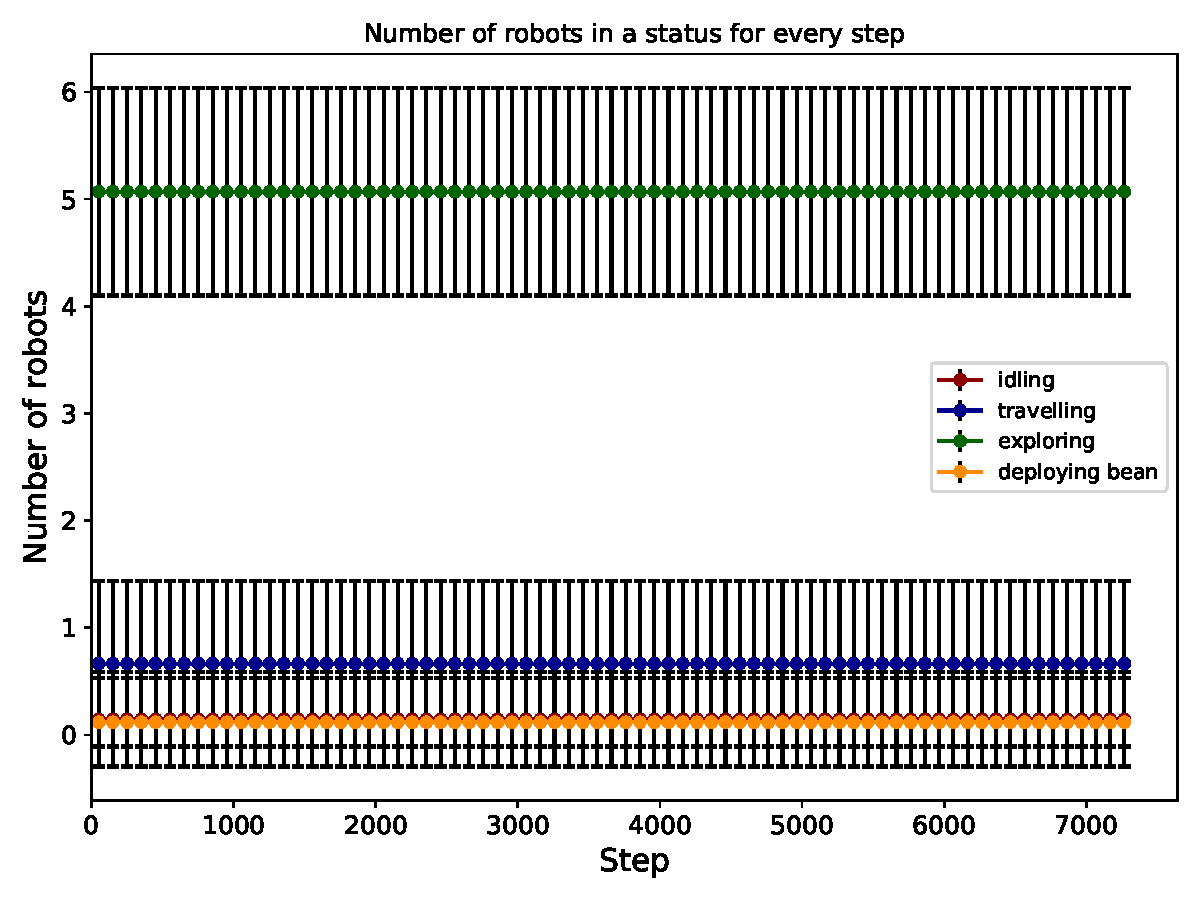
\includegraphics[width = .5\textwidth]{images/status_results/random1_sim0}} &
		\subfloat[Stato dei robot durante l'esplorazione della mappa generata casualmente numero 3.]{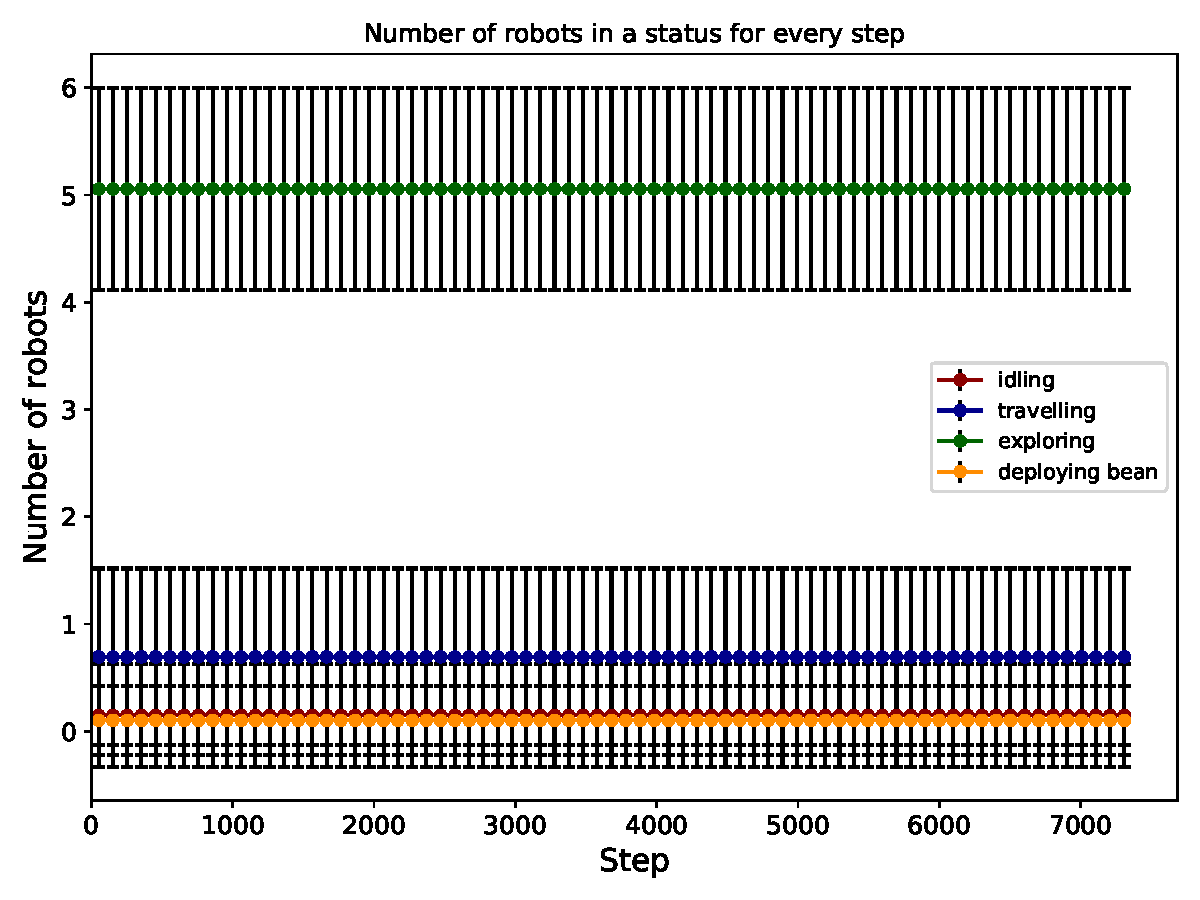
\includegraphics[width = .5\textwidth]{images/status_results/random3_sim0}}\\
	\end{tabular}
		\centering
		\subfloat[Stato dei robot durante l'esplorazione della mappa generata casualmente numero 4.]{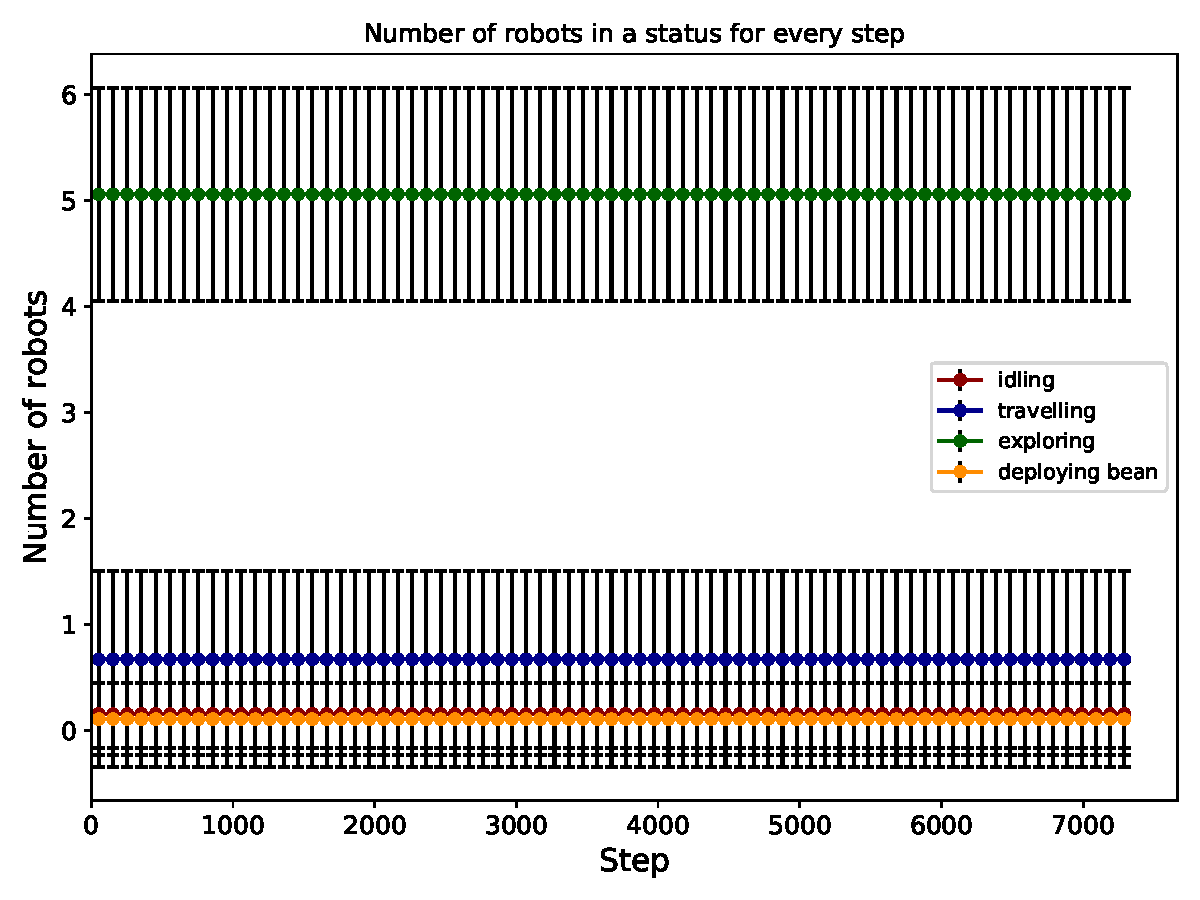
\includegraphics[width = .5\textwidth]{images/status_results/random4_sim0}}
	\caption{Sull'asse delle \textit{x} si trova il tempo, in termini di \textit{step}, impiegato per l'esplorazione della mappa, mentre sull'asse delle \textit{y} il numero di agenti in un determinato stato. Si noti che i dati sono stati raggruppati per formare 100 \textit{bin} in modo da rendere leggibile il grafico; di conseguenza, in colore si trovano le medie e le \textit{errorbar} rappresentano le devizioni standard rispeto alla media.}
	\label{figapx:status}
\end{figure}